\documentclass{article}
\usepackage[utf8]{inputenc}
\usepackage{amsmath}
\usepackage{graphicx}
\graphicspath{ {images/} }

\title{Componenti fortemente connesse di grafi}
\author{Marco Benelli}
\date{Settembre 2019}

\begin{document}

\maketitle

\section{Introduzione}

L'obiettivo è misurare la velocità e la complessità dell'algoritmo per trovare le componenti fortemente connesse di un grafo e verificare che queste siano coerenti con i risultati teorici.

\section{Teoria}

L'algoritmo ha un costo asintotico del tipo $\Theta(V + E) = O(V^2)$ poiché $E = O(V^2)$.

\section{Prestazioni attese}

Le complessità di cui si è parlato nella sezione precedente sono da intendersi come asintotiche. I tempi di esecuzione possono avere un andamento diverso per grafi piccoli. Quello che speriamo è che raggiungano un andamento simile a quello teorico anche per grafi relativamente piccoli.

\section{Esperimenti}

Verranno svolti due esperimenti: uno su grafi che hanno un numero di archi pari al numero di vertici ($E = V = \Theta(V)$) e uno su grafi che hanno un numero di archi pari alla metà del massimo possibile ($E = \frac{V^2}{2} = \Theta(V^2)$). Gli esperimenti verranno condotti su grafi di grandezza sempre crescente (ogni volta la grandezza viene raddoppiata) finché il tempo di esecuzione non supera i 256 secondi. Per ogni numero di nodi e per ogni numero di archi vengono condotti 16 test e viene fatta la media fra i loro tempi di esecuzione.

\section{Codice}

Il codice è diviso in tre sezioni: le classi che implementano i grafi e i loro metodi (queste sono semplicemente delle traduzioni in Python dello pseudo codice visto a lezione), le funzioni che implementano i test e le funzioni che disegnano i grafici.

Per misurare i tempi di esecuzione si usa la funzione default timer dal modulo timeit della libreria standard di Python.

Per quanto riguarda i grafici, si usa la libreria matplotlib, nello specifico il modulo pyplot. I vettori che vengono dati alla funzione plot sono il vettore delle grandezza dei grafi (come vettore delle x) e il vettore dei tempi di esecuzione (come vettore delle y) per ogni test. Oltre a queste due curve, vengono anche disegnate altre due curve che indicano l'andamento predetto dalla teoria per confrontarlo con l'andamento sperimentale.

\section{Risultati sperimentali}

\begin{figure}[h]
    \centering
    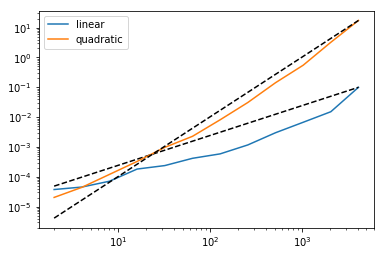
\includegraphics{grafico}
    \caption{I risultati del test}
    \label{fig:grafico}
\end{figure}

Nella figura \ref{fig:grafico} possiamo vedere che i risultati sperimentali sono in linea con le predizioni teoriche visto che le linee colorate si sovrappongono a quelle tratteggiate. È importante notare che il grafico è in scala logaritmica, in modo che complessità lineari e complessità quadratiche possano essere rappresentate con rette. Le linee tratteggiate indicano l'andamento teorico e sono ottenute moltiplicando la funzione teorica per un coefficiente opportuno. Questo coefficiente si trova imponendo che la linea tratteggiata e quella colorata abbiano in comune l'ultimo punto.

Questi risultati ci portano a concludere che per sfruttare al meglio la velocita della depth-first search (e quindi dell'algoritmo per trovare le componenti fortemente connesse) è importante (specialmente nei grafi con pochi archi) implementare il grafo tramite liste di adiacenza, altrimenti la complessità diventerebbe $\Theta(V^2)$.

\end{document}
